\documentclass[12pt, letterpaper]{article}

\usepackage{../../spreamble}
\usepackage{graphicx}

\title{COP3530 - Project 1 Check-in}
\author{Ian Zou}

\begin{document}

\part*{The Code}

\maketitle
\begin{minted}[
        linenos,
        frame=lines,
        framesep=2mm,
        baselinestretch=1.2,
        breaklines,
        mathescape,
]
{cpp}
/* Ian Zou - 69896641 */
#include <catch2/catch_test_macros.hpp>
#include <random>
#include <set>

#include "./avl-tree.hpp"

TEST_CASE("Invalid Command Executions", "[frontend]") {
    std::stringstream out;

    parse(out, "insert A11y 45679999");
    REQUIRE(out.str() == "unsuccessful");

    parse(out, "insert Bob 22222");
    REQUIRE(out.str() == "unsuccessful");
    
    parse(out, "search 2");
    REQUIRE(out.str() == "unsuccessful");

    parse(out, "remove Bob");
    REQUIRE(out.str() == "unsuccessful");

    parse(out, "remove 22222");
    REQUIRE(out.str() == "unsuccessful");
}

TEST_CASE("Left-Left Case Rotation", "[AVLTree]") {
    AVLTree<int> tree;

    tree.insert(3);
    tree.insert(2);
    tree.insert(1);

    REQUIRE(tree.height(tree.root) == 2);

    REQUIRE(tree.root->val == 2);
    REQUIRE(tree.root->left->val == 1);
    REQUIRE(tree.root->right->val == 3);
}

TEST_CASE("Right-Right Case Rotation", "[AVLTree]") {
    AVLTree<int> tree;

    tree.insert(1);
    tree.insert(2);
    tree.insert(3);

    REQUIRE(tree.height(tree.root) == 2);

    REQUIRE(tree.root->val == 2);
    REQUIRE(tree.root->left->val == 1);
    REQUIRE(tree.root->right->val == 3);
}

TEST_CASE("Left-Right Case Rotation", "[AVLTree]") {
    AVLTree<int> tree;

    tree.insert(3);
    tree.insert(1);
    tree.insert(2);

    REQUIRE(tree.height(tree.root) == 2);

    REQUIRE(tree.root->val == 2);
    REQUIRE(tree.root->left->val == 1);
    REQUIRE(tree.root->right->val == 3);
}

TEST_CASE("Right-Left Case Rotation", "[AVLTree]") {
    AVLTree<int> tree;

    tree.insert(3);
    tree.insert(2);
    tree.insert(1);

    REQUIRE(tree.height(tree.root) == 2);

    REQUIRE(tree.root->val == 2);
    REQUIRE(tree.root->left->val == 1);
    REQUIRE(tree.root->right->val == 3);
}

TEST_CASE("Insertion and Removal", "[AVLTree]") {
    AVLTree<int> tree;

    for (size_t i = 1; i <= 100; ++i) {
        tree.insert(static_cast<int>(i));
    }

    std::mt19937 rand(static_cast<unsigned long>(time(nullptr)));
    std::set<int> set;

    while (set.size() < 10) {
        int s = (rand() % 100) + 1;

        if (set.count(s) == 0) {
            set.emplace(s);
        }
    }

    for (auto begin = set.begin(); begin != set.end(); ++begin) {
        auto node = tree.search(*begin);
        tree.remove(node);
    }

    tree.inorder_traversal([&set](Node<int>* node) {
        REQUIRE(set.count(node->val) == 0);
    });
}

TEST_CASE("Inorder Traversal", "[AVLTree]") {
    AVLTree<int> tree;

    tree.insert(3);
    tree.insert(1);
    tree.insert(5);
    tree.insert(2);
    tree.insert(4);

    const std::vector<int> correct = { 1, 2, 3, 4, 5 };
    std::vector<int> traversal;
    tree.inorder_traversal([&traversal] (Node<int>* node) {
            traversal.emplace_back(node->val);
    });
    
    REQUIRE(traversal == correct);
}
\end{minted}

\part{The Screenshot}

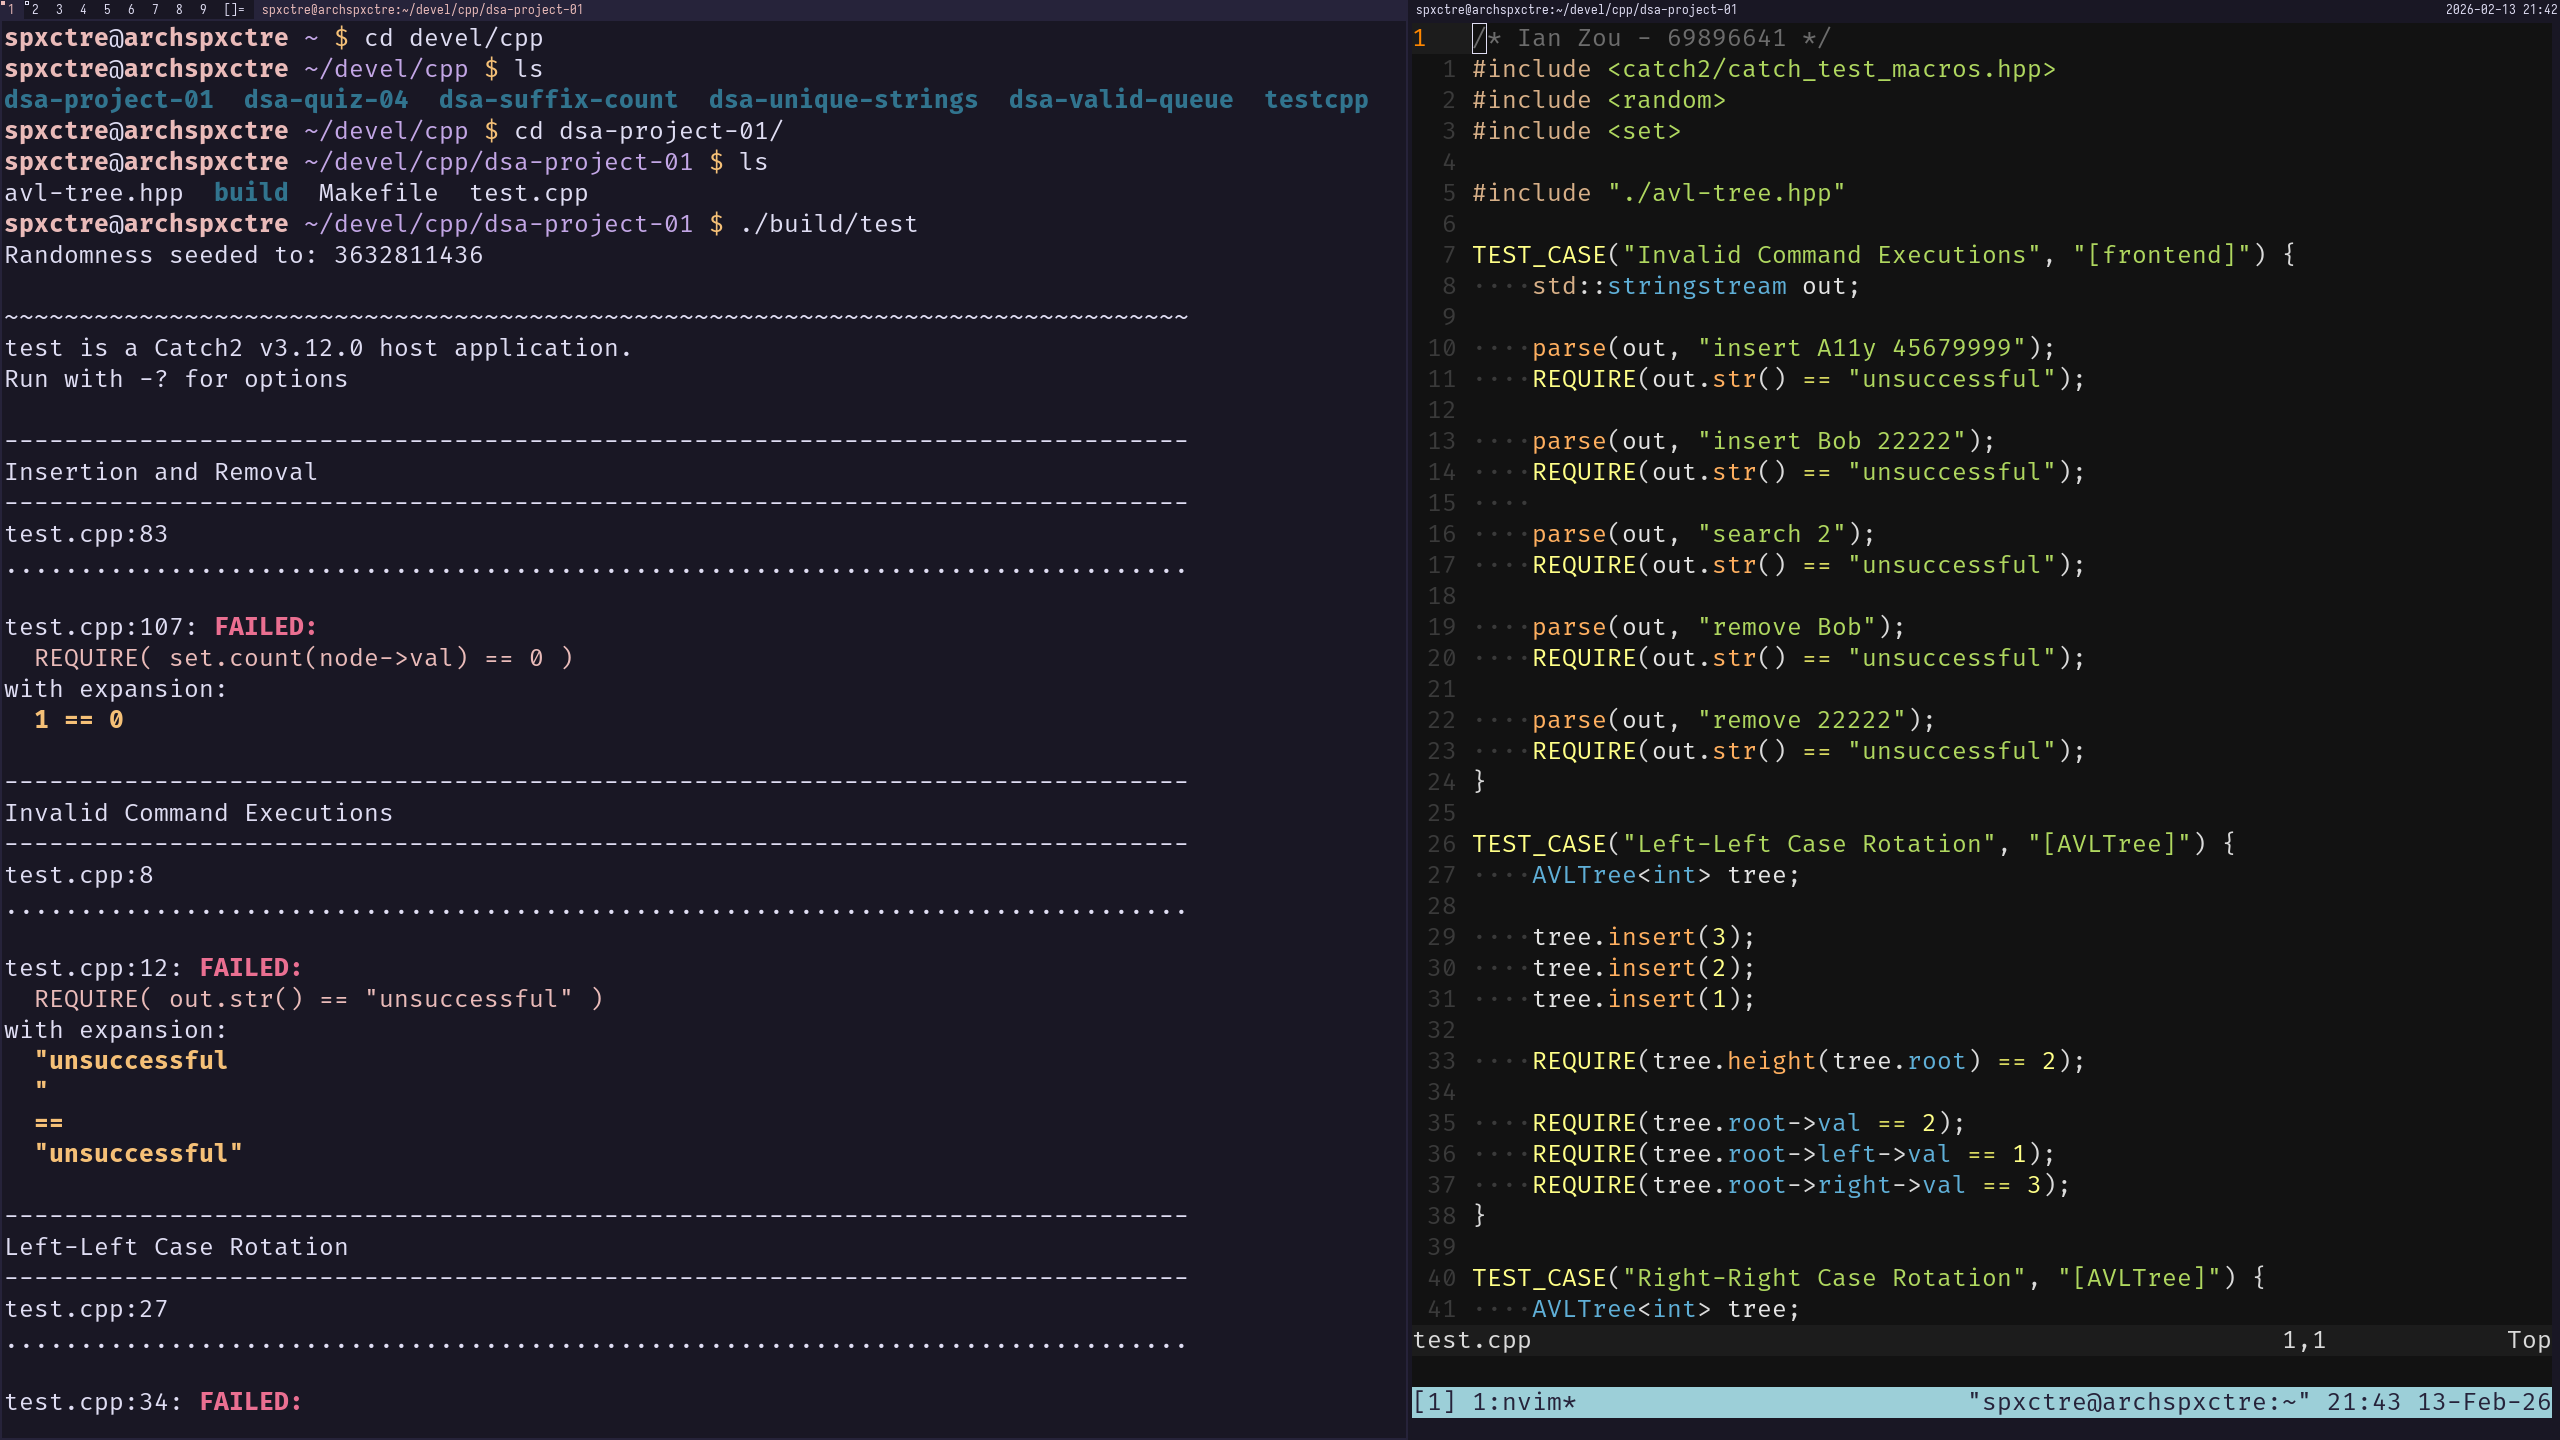
\includegraphics[width=\textwidth]{./project1checkin.png}

\end{document}

